\setchapterpreamble[u]{\margintoc}
\chapter{Autenticazione utente}
\labch{chapter4}

Autenticazione utente:
\begin{itemize}
    \item Processo per determinare se un utente o qualche applicazione o processo che agisce per conto di un utente è, in effetti, chi o cosa dichiara di essere;
	\item La tecnologia di autenticazione fornisce il controllo dell'accesso ai sistemi controllando se le credenziali di un utente corrispondono alle credenziali in un database di utenti autorizzati o in un server di autenticazione dati;
	\item L'autenticazione consente alle organizzazioni di proteggere le proprie reti consentendo solo agli utenti (o processi) autenticati di accedere alle risorse protette;
	\item L'autenticazione dell'utente è distinta dall'autenticazione del messaggio: l'autenticazione del messaggio è una procedura che consente alle parti comunicanti di verificare che il contenuto di un messaggio ricevuto non sia stato alterato e che la fonte sia autentica.
\end{itemize}

Principi dell'autenticazione:
\begin{itemize}
    \item \textbf{Identità digitale}: rappresentazione unica di un soggetto impegnato in una transazione online. Consiste in un attributo o insieme di attributi che descrivono in modo univoco un soggetto all'interno di un dato contesto di un servizio digitale, ma non identificano necessariamente in modo univoco il soggetto in tutti i contesti;
	\item \textbf{Prova dell'identità}: stabilisce che un soggetto è chi afferma di essere ad un determinato livello di certezza. Consiste nella raccolta delle info sull'utente e la creazione della sua identità (primo accesso);
	\item \textbf{Autenticazione digitale}: processo di determinazione della validità di uno o più autenticatori utilizzati per rivendicare un'identità digitale. La riuscita dell'autenticazione fornisce garanzie ragionevoli basate sul rischio che il soggetto che accede al servizio oggi è lo stesso del soggetto che ha precedentemente effettuato l'accesso al servizio (dal secondo accesso in poi).
\end{itemize}

Mezzi di autenticazione:
\begin{itemize}
    \item Qualcosa che si conosce;
	\item Qualcosa che si possiede;
	\item Qualcosa che si è o si fa;
\end{itemize}

\section{Autenticazione reciproca}
I protocolli che consentono alle parti comunicanti di soddisfarsi reciprocamente sull'identità dell'altro e di scambiare chiavi di sessione devono gestire due problematiche:
\begin{itemize}
    \item \textbf{Riservatezza}: info sull'identità e sulle chiavi di sessione devono essere scambiate in forma cifrata. Questo richiede la preventiva esistenza di chiavi segrete o pubbliche utilizzabili a tale scopo;
	\item \textbf{Tempestività}: importante a causa della minaccia di ripetizioni dei messaggi. I replay potrebbero permettere all'attaccante di:
	\begin{itemize}
	    \item Compromettere una chiave di sessione;
		\item Impersonare con successo l'altra parte;
		\item Interrompere le operazioni presentando alle parti messaggi che sembrano autentici ma non lo sono.
	\end{itemize}
\end{itemize}

Possibili replay attack:
\begin{itemize}
    \item L'attacco più semplice è quello in cui l'avversario copia semplicemente un messaggio e lo riproduce in seguito:
	\item Un avversario può riprodurre un messaggio con timestamp entro la finestra temporale valida;
	\item Un avversario può riprodurre un messaggio con timestamp entro la finestra temporale valida, ma in aggiunta, l'avversario sopprime il messaggio originale; quindi, la ripetizione non può essere rilevata;
	\item Un altro attacco prevede un replay all'indietro senza modifica ed è possibile se viene utilizzata la crittografia simmetrica e il mittente non può riconoscere facilmente la differenza tra messaggi inviati e messaggi ricevuti in base al contenuto (reflection attack).
\end{itemize}

Protezione dai replay attack:
\begin{itemize}
    \item Aggiungere un sequence number a ciascun messaggio utilizzato in uno scambio di autenticazione. Un nuovo messaggio viene accettato solo se il numero di sequenza è nell'ordine corretto. La difficoltà con questo approccio è che richiede a ciascuna parte di tenere traccia dell'ultimo numero di sequenza per ogni altra parte con cui ha avuto a che fare. Generalmente non è usato nell'autenticazione e nello scambio delle chiavi perché genera overhead;
	\item Aggiungere un timestamp. Richiede la sincronizzazione degli orologi tra i vari partecipanti. A accetta il messaggio solo se il timestamp rientra nel tempo di attesa accettato;
	\item Usare una challenge-response. A invia un nonce a B (challenge) e si aspetta che la risposta di B lo contenga (response).
\end{itemize}

\underline{Suppress Replay Attack}: Il protocollo di Denning richiede l'utilizzo di orologi sincronizzati in tutta la rete. È un vincolo rischioso in quanto gli orologi distribuiti possono non sincronizzarsi a causa di sabotaggi o guasti negli orologi stessi o nel meccanismo di sincronizzazione. Il problema si verifica quando l'orologio di un mittente è in anticipo rispetto all'orologio del destinatario: l'attaccante può intercettare il messaggio, catturarlo e rinviarlo quando il timestamp del messaggio è sincronizzato con l'orologio del ricevente.

Autenticazione remota dell'utente con chiave simmetrica:
\begin{itemize}
    \item È possibile utilizzare una gerarchia a due livelli di chiavi simmetriche per garantire la riservatezza per le comunicazioni in un ambiente distribuito;
	\item La strategia prevede l'uso di un centro di distribuzione delle chiavi affidabile (KDC);
	\item Ciascuna parte condivide una chiave segreta, nota come master key, con il KDC;
	\item Il KDC ha il compito di generare e distribuire le chiavi temporanee usate nella connessione. Le distribuzione delle chiavi temporanee viene protetta usando le master key.
\end{itemize}

\section{Kerberos}

Servizio di autenticazione sviluppato nell'ambito del Progetto Athena al MIT. Si basa sul concetto che non ci si può fidare di una workstation per identificare correttamente i suoi utenti per l'accesso ai servizi di rete:
\begin{itemize}
    \item Un utente può accedere a una determinata workstation e fingere di essere un altro utente che opera da quella workstation;
	\item Un utente può modificare l'indirizzo di rete di una workstation in modo che le richieste inviate dalla workstation modificata sembrino provenire dalla workstation rappresentata;
	\item Un utente può intercettare gli scambi e utilizzare un replay attack per accedere a un server o interrompere le operazioni.
\end{itemize}

Kerberos fornisce un server di autenticazione centralizzato la cui funzione consiste nell'autenticare gli utenti sui server e i server sugli utenti. Utilizza solo crittografia simmetrica (no chiavi pubbliche).

Requisiti:
\begin{itemize}
    \item Sicuro: un intercettatore sulla rete non dovrebbe essere in grado di ottenere le informazioni necessarie per impersonare un utente;
	\item Affidabile: dovrebbe essere altamente affidabile e dovrebbe impiegare un'architettura a server distribuiti con un sistema in grado di eseguire il backup di un altro;
	\item Trasparente: idealmente, l'utente non dovrebbe essere consapevole del fatto che l'autenticazione sta avvenendo oltre al requisito di immissione di una password;
	\item Scalabile: il sistema dovrebbe essere in grado di supportare un numero elevato di client e server.
\end{itemize}

\subsection{Kerberos v.4 (1988)}

Utilizza DES per fornire il servizio di autenticazione.

Componenti:
\begin{enumerate}
    \item Server di autenticazione (AS): conosce le password di tutti gli utenti e le archivia in modo centralizzato. Condivide una chiave univoca con ogni server;
	\item Ticket generale: creato una volta che l'AS accetta l'utente come autentico; contiene l'ID dell'utente e l'indirizzo di rete e l'ID del server-granting ticket (TGS). Il ticket è cifrato usando la chiave condivisa tra l'AS e quel TGS;
	\item Ticket-granting server (TGS): emette ticket specifici per permette all'utente di accedere ai servizi. Ogni volta che l'utente deve accedere ad un servizio, presenta al TGS il ticket generale ricevuto dall'AS. Il TGS verifica il ticket e genera un ticket specifico che l'utente userà per autenticarsi al server che gestisce il servizio/risorsa che ha richiesto.
\end{enumerate}
	
Problemi da tener presente nello scambio dei messaggi:
\begin{itemize}
    \item La durate del ticket generale può essere un problema:
	\begin{itemize}
	    \item Se la durata è molto breve (es. minuti), all'utente verrà ripetutamente richiesta una password (deve riautenticarsi con l'AS);
		\item Se la vita è lunga (ad esempio, ore), allora aumentano le possibilità di un replay attack.
	\end{itemize}
	\item Un servizio di rete (il TGS o un servizio applicativo) deve essere in grado di provare che la persona che utilizza un biglietto è la stessa persona a cui è stato emesso quel biglietto (utilizzare un autenticatore).
	\item Inoltre i server devono autenticarsi agli utenti (tramite un secondo autenticatore).
\end{itemize}

Scambio dei messaggi (figura \ref{fig:4-1}):
\begin{enumerate}
    \item Il client contatta l'AS per richiedere l'accesso al servizio del TGS;
	\begin{itemize}
	    \item Messaggio = [ID client, ID TGS, timestamp1]
	\end{itemize}
	\item L'AS invia il ticket generale al client. Il messaggio è cifrato con una chiave che l'AS deriva dalla password del client (che conosce). Ricevuto il messaggio il client calcolerà la chiave a partire dalla chiave passata dall'utente: 
	\begin{itemize}
	    \item Messaggio = [ID TGS, timestamp2, ticket generale]
		\item Ticket = [chiave di sessione per client e TGS, ID client, indirizzo client, ID TGS, timestamp2, tempo di vita del ticket]
		\begin{itemize}
		    \item Ticket cifrato con la chiave condivisa tra TGS e AS
		\end{itemize}
	\end{itemize}
	\item Il client contatta il TGS per richiedere l'accesso al servizio;
	\begin{itemize}
	    \item Messaggio = [ID client, ticket generale, autenticatore]
		\item Autenticatore = [ID client, indirizzo client, timestamp4]
	\end{itemize}
	\item Il TGS fornisce al client il ticket per accedere al server che gestisce il servizio;
	\begin{itemize}
	    \item Messaggio = [chiave di sessione generata dal TGS per la comunicazione tra client e server, ID client, timestamp4, ticket]
		\begin{itemize}
		    \item Messaggio cifrato con chiave di sessione client-TGS
		\end{itemize}
		\item Ticket = [chiave di sessione client-server, ID client, indirizzo client, ID server, timestamp4, tempo di vita del ticket]
		\begin{itemize}
		    \item Ticket cifrato con una chiave conosciuta solo da serve e TGS, per evitare tampering
		\end{itemize}
	\end{itemize}
	\item Il client invia il ticket al server per richiedere l'accesso alla risorsa;
    \begin{itemize}
        \item Messaggio = [ticket, autenticatore]
		\item Autenticatore = [ID client, indirizzo client, timestamp5]
		\begin{itemize}
		    \item Autenticatore cifrato con la chiave di sessione client-server
		\end{itemize}
    \end{itemize}
	\item Se è richiesta la mutua autenticazione, il server risponde al client autenticandosi.
	\begin{itemize}
	    \item Messaggio = [timestamp5 incrementato di 1]
		\begin{itemize}
		    \item Messaggio cifrato con la chiave di sessione client-server
		\end{itemize}
	\end{itemize}
\end{enumerate}

\begin{figure}
    \centering
    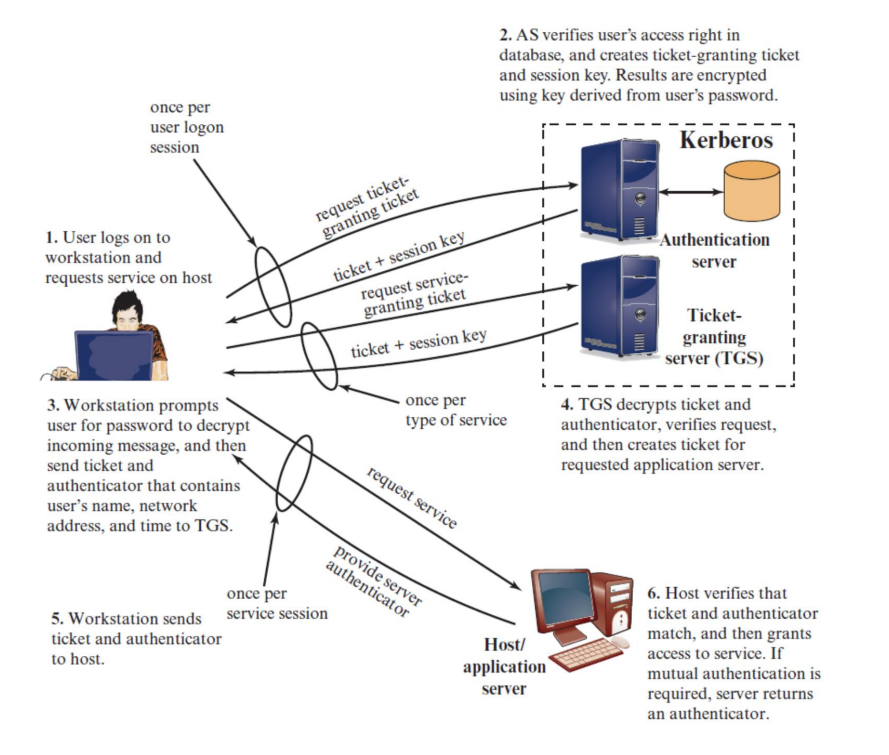
\includegraphics[width=1\textwidth]{images/chapter4/4-1.png}
    \caption{Scambio dei messaggi.}
    \label{fig:4-1}
\end{figure}

\subsection{Reami di kerberos}

Un ambiente full-service di kerberos comprende Il server Kerberos, un certo numero di client e un certo numero di server delle applicazioni. Questo tipo di ambiente vuole che:
\begin{itemize}
    \item Il server Kerberos deve avere l'ID utente e l'hash delle password di tutti gli utenti partecipanti nel suo database. Tutti gli utenti sono registrati col server Kerberos;
	\item Il server Kerberos deve condividere una chiave segreta con ciascun server TGS. Tutti i server sono registrati col server Kerberos;
	\item Il server TGS di ogni reame condivide una chiave segreta con ogni altro TGS di ogni altro reame. In questo modo le coppie di TGS si autenticano tra loro permettendo ad un utente del reame A di richiedere servizi al reame B interfacciandosi col TGS di B. Presenterà quindi a B un ticket per "risorsa esterna" emesso dal TGS di A. Il TGS di B accetterà la richiesta, rilasciando un nuovo ticket, in quanto si fida del TGS di A.
	Il ticket che il TGS di A dà al client contiene la chiave segreta condivisa tra i due TGS.
\end{itemize}
	
Il numero di chiavi condivise tra i TGS è n(n-1). Supponendo che i TGS siano 3, ogni TGS condivide 2 chiavi con gli altri, quindi il numero di chiavi totali è 6. 
Il numero limitato di chiavi e la possibilità di avere reami rendono kerberos scalabile.

\subsection{Differenze tra kerberos 4 e 5}

La versione 5 risolve alcune limitazioni della 4:
\begin{enumerate}
    \item Limiti sull'ambiente:
	\begin{itemize}
	    \item Utilizzo di AES per la cifratura (al posto di DES);
		\item Dipendenza dal protocollo Internet (non solo indirizzi IP, eventuali indirizzi di rete);
		\item Ordinamento dei byte del messaggio;
		\item Durata del ticket (durata con ora di inizio e fine esplicita nei ticket);
		\item Inoltro dell'autenticazione (visto che sono autenticato per l'uso della stampante, sono autenticato anche per le risorse che la stampante usa);
		\item Autenticazione Inter-reame (un metodo che richiede meno di $O(n^2)$ chiavi);
	\end{itemize}
    \item Limiti tecnici:
    \begin{itemize}
        \item Rimozione della doppia cifratura (analisi hanno dimostrato che non è necessario, si rimuove perché pesante);
		\item Aggiunto meccanismo di integrità:
		\item Le chiavi di sotto-sessione possono essere negoziate solo per una connessione;
		\item Preautenticazione per prevenire attacchi alle password.
    \end{itemize}
\end{enumerate}

\underline{Autenticazione mutuale}: si usa la cifratura a chiave pubblica per la distribuzione delle chiavi di sessione. La distribuzione avviene col protocollo di Dennign esteso con timestamp.

Autenticazione one-way: 
\begin{itemize}
    \item Riguarda un unico trasferimento di informazioni da un utente A ad un utente B;
	\item Stabilisce un flusso da A a B con un qualcosa che autentica il mittente;
	\item Per garantire la riservatezza il Messaggio è cifrato con una chiave one-time;
	\item La chiave one-time viene cifrata con la chiave pubblica di B, quindi solo B è in grado di recuperare la chiave e decifrare il messaggio;
	\item Questo schema (chiave one-time cifrata con chiave pubblica di B, messaggio cifrato con chiave one-time) è più efficiente che cifrare l'intero messaggio con la chiave pubblica di B;
\end{itemize}

Se mi preoccupa l'autenticazione, posso usare la firma digitale. Questo metodo garantisce che A non possa negare in seguito di aver inviato il messaggio (ma potrebbe essere che A non sia il vero originatore del massaggio). Quindi:
\begin{itemize}
    \item Oltre la messaggio, A invia a B la firma cifrata con la chiave privata di A e il certificato di A cifrato con la chiave privata dell'AS;
	\item B usa il certificato di A per ottenere la chiave pubblica di A e verifica che sia autentica;
	\item B usa quindi la chiave per verificare il messaggio;
\end{itemize}

Se è richiesta anche la confidenzialità, l'intero massaggio viene cifrato con la chiave pubblica di B oppure con una chiave one-time che viene cifrata con la chiave pubblica di B.

\section{Identità federata}
Identità comune in più aziende e numerose applicazioni. Fornisce diversi servizi come:
\begin{itemize}
    \item Punto di contatto;
	\item Servizi del protocollo SSO;
	\item Servizi fiduciari;
	\item Servizi di chiavi;
	\item Servizi di identità;
	\item Autorizzazioni;
	\item Gestione.
\end{itemize}

La gestione dell'identità consiste in un approccio centralizzato e automatizzato per fornire l'accesso alle risorse a livello aziendale da parte dei dipendenti e di altre persone autorizzate. L'obiettivo della gestione dell'identità è definire un'identità per ciascun utente (umano o processo), associare attributi all'identità e applicare un mezzo attraverso il quale un utente può verificare l'identità. Il concetto centrale del sistema è l'uso del single sign-on (SSO), che consente ad un utente di accedere a tutte le risorse di rete dopo un'unica autenticazione (figura \ref{fig:4-2}).

\begin{figure}
    \centering
    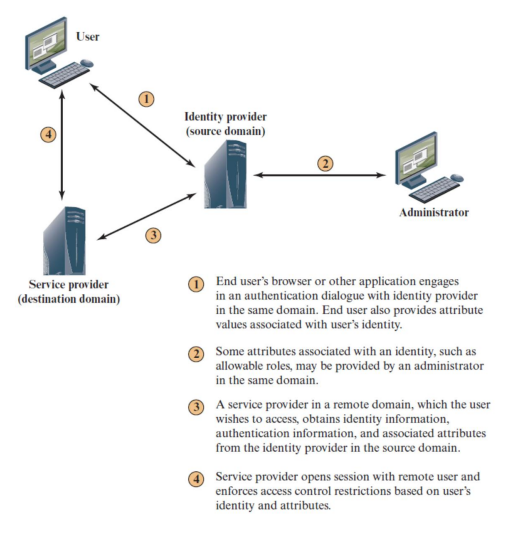
\includegraphics[width=1\textwidth]{images/chapter4/4-2.png}
    \caption{Identità federata.}
    \label{fig:4-2}
\end{figure}